% Options for packages loaded elsewhere
\PassOptionsToPackage{unicode}{hyperref}
\PassOptionsToPackage{hyphens}{url}
%
\documentclass[
]{book}
\usepackage{lmodern}
\usepackage{amssymb,amsmath}
\usepackage{ifxetex,ifluatex}
\ifnum 0\ifxetex 1\fi\ifluatex 1\fi=0 % if pdftex
  \usepackage[T1]{fontenc}
  \usepackage[utf8]{inputenc}
  \usepackage{textcomp} % provide euro and other symbols
\else % if luatex or xetex
  \usepackage{unicode-math}
  \defaultfontfeatures{Scale=MatchLowercase}
  \defaultfontfeatures[\rmfamily]{Ligatures=TeX,Scale=1}
\fi
% Use upquote if available, for straight quotes in verbatim environments
\IfFileExists{upquote.sty}{\usepackage{upquote}}{}
\IfFileExists{microtype.sty}{% use microtype if available
  \usepackage[]{microtype}
  \UseMicrotypeSet[protrusion]{basicmath} % disable protrusion for tt fonts
}{}
\makeatletter
\@ifundefined{KOMAClassName}{% if non-KOMA class
  \IfFileExists{parskip.sty}{%
    \usepackage{parskip}
  }{% else
    \setlength{\parindent}{0pt}
    \setlength{\parskip}{6pt plus 2pt minus 1pt}}
}{% if KOMA class
  \KOMAoptions{parskip=half}}
\makeatother
\usepackage{xcolor}
\IfFileExists{xurl.sty}{\usepackage{xurl}}{} % add URL line breaks if available
\IfFileExists{bookmark.sty}{\usepackage{bookmark}}{\usepackage{hyperref}}
\hypersetup{
  pdftitle={From Scratch},
  pdfauthor={Patrick Altmeyer},
  hidelinks,
  pdfcreator={LaTeX via pandoc}}
\urlstyle{same} % disable monospaced font for URLs
\usepackage{longtable,booktabs}
% Correct order of tables after \paragraph or \subparagraph
\usepackage{etoolbox}
\makeatletter
\patchcmd\longtable{\par}{\if@noskipsec\mbox{}\fi\par}{}{}
\makeatother
% Allow footnotes in longtable head/foot
\IfFileExists{footnotehyper.sty}{\usepackage{footnotehyper}}{\usepackage{footnote}}
\makesavenoteenv{longtable}
\usepackage{graphicx,grffile}
\makeatletter
\def\maxwidth{\ifdim\Gin@nat@width>\linewidth\linewidth\else\Gin@nat@width\fi}
\def\maxheight{\ifdim\Gin@nat@height>\textheight\textheight\else\Gin@nat@height\fi}
\makeatother
% Scale images if necessary, so that they will not overflow the page
% margins by default, and it is still possible to overwrite the defaults
% using explicit options in \includegraphics[width, height, ...]{}
\setkeys{Gin}{width=\maxwidth,height=\maxheight,keepaspectratio}
% Set default figure placement to htbp
\makeatletter
\def\fps@figure{htbp}
\makeatother
\setlength{\emergencystretch}{3em} % prevent overfull lines
\providecommand{\tightlist}{%
  \setlength{\itemsep}{0pt}\setlength{\parskip}{0pt}}
\setcounter{secnumdepth}{5}
\usepackage{booktabs}
\usepackage{amsthm}
\makeatletter
\def\thm@space@setup{%
  \thm@preskip=8pt plus 2pt minus 4pt
  \thm@postskip=\thm@preskip
}
\makeatother
\usepackage[]{natbib}
\bibliographystyle{apalike}

\title{From Scratch}
\usepackage{etoolbox}
\makeatletter
\providecommand{\subtitle}[1]{% add subtitle to \maketitle
  \apptocmd{\@title}{\par {\large #1 \par}}{}{}
}
\makeatother
\subtitle{Data Science from a student's perspective}
\author{Patrick Altmeyer}
\date{2020-10-13}

\begin{document}
\maketitle

{
\setcounter{tocdepth}{1}
\tableofcontents
}
\hypertarget{intro}{%
\chapter{Introduction}\label{intro}}

\hypertarget{det-opt}{%
\chapter{Deterministic optimization}\label{det-opt}}

\hypertarget{line-search}{%
\section{Line search}\label{line-search}}

\hypertarget{methodology}{%
\subsection{Methodology}\label{methodology}}

The goal of Exercise 3.1 in \citet{nw2006numerical} is to minimize the bivariate Rosenbrock function (Equation \eqref{eq:rosenbrock}) using \emph{steepest descent} and \emph{Newton's method}. The Rosenbrock function - also known as \emph{Rosenbrock's banana function} - has a long, narrow, parabolic shaped flat valley and is often used for to test optimization algorithms for their performance (see \href{https://en.wikipedia.org/wiki/Rosenbrock_function}{here}).

\[
\begin{equation}
  f(\mathbb{x})=100(x_2-x_1^2)^2+(1-x_1)^2 
  \label{eq:rosenbrock}
\end{equation}
\]
We can implement Equation \eqref{eq:rosenbrock} in R as follows:

Figure \ref{fig:rosenbrock} shows the output of the function over \(x_1,x_2 \in [-1.5, 1.5]\) along with its minimum indicated as a red asterisk and the two starting points: (1) \(X_0=(1.2,1.2)\) and (2) \(X_0=(-1.2,1)\).

\begin{figure}
\centering
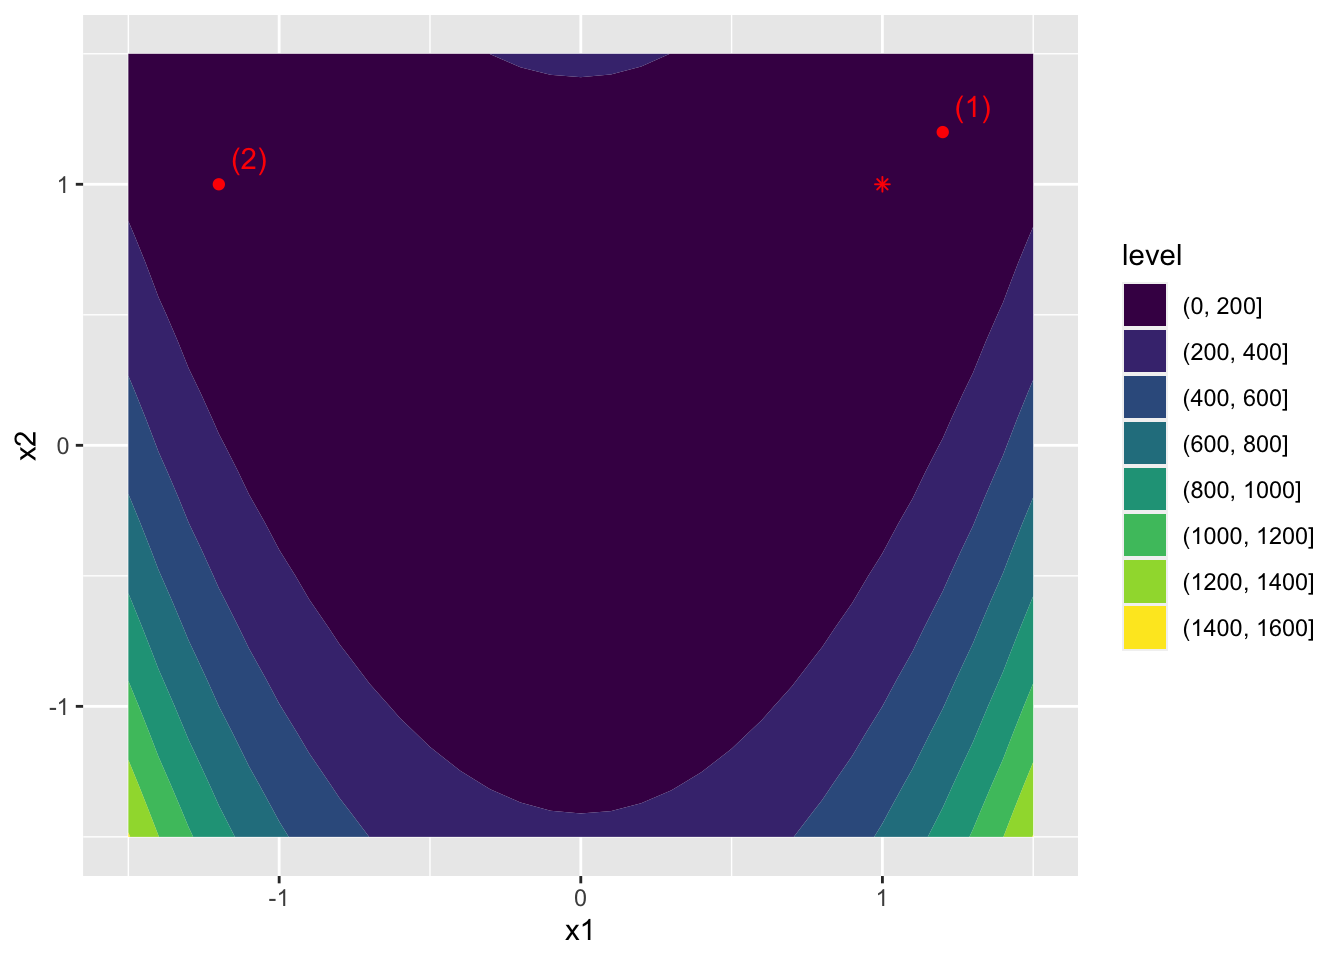
\includegraphics{fromScratch_files/figure-latex/rosenbrock-1.pdf}
\caption{\label{fig:rosenbrock}Output of the Rosenbrock function and minimizer in red.}
\end{figure}

The gradient and Hessian of \(f\) can be computed as

\[
\begin{equation}
\nabla f(\mathbb{x})= \begin{pmatrix}
\frac{ \partial f}{\partial x_1} \\
\frac{ \partial f}{\partial x_2}
\end{pmatrix} 
\label{eq:d-rosenbrock}
\end{equation}
\]

and

\[
\begin{equation}
\nabla^2 f(\mathbb{x})= \begin{pmatrix}
\frac{ \partial^2 f}{\partial x_1^2} & \frac{ \partial^2 f}{\partial x_1 \partial x_2} \\
\frac{ \partial^2 f}{\partial x_2\partial x_1} & \frac{ \partial^2 f}{\partial x_2^2}
\end{pmatrix}
\label{eq:dd-rosenbrock}
\end{equation}
\]

which in R can be encoded as follows:

For both methods I will use the \emph{Arminjo condition} with backtracking. The \texttt{gradient\_desc} function (below) can implement both \emph{steepest descent} and \emph{Newton's method}. The code for the function can be inspected below (you can reveal it by simply clicking on the \emph{Code} button on the right). There's also a small description of the different arguments.

Similarly you can take a look at how the \texttt{gradient\_desc} is applied in the underlying problem by unhiding the next code chunk.

\hypertarget{results}{%
\subsection{Results}\label{results}}

The below shows how the two algorithms converge to

  \bibliography{bib.bib,packages.bib}

\end{document}
